\documentclass[conference]{IEEEtran}
\IEEEoverridecommandlockouts

\usepackage[T1]{fontenc}
\usepackage{cite}
\usepackage{amsmath,amssymb}
\usepackage{graphicx}
\usepackage{booktabs}
\usepackage{array}
\usepackage{multirow}
\usepackage{algorithm}
\usepackage{algpseudocode}
\usepackage{tikz}
\usetikzlibrary{positioning,arrows.meta,fit,calc}
\usepackage{pgfplots}
\pgfplotsset{compat=1.18}
\usepackage{xcolor}
\usepackage[hidelinks]{hyperref}

\begin{document}

\title{Wardrobe+: A Smartphone Wardrobe Assistant with Garment Classification, Colour Detection and Explainable Outfit Recommendation}

\author{
\IEEEauthorblockN{Manaswi Bajaj, Atharva Bhargava, Harsh Doshi, Khush Doshi}
\IEEEauthorblockA{Department of Information Technology\\
Dwarkadas J. Sanghvi College of Engineering, University of Mumbai, Mumbai, India\\
Guide: Prof. Neha Ram}
}

\maketitle

\begin{abstract}
People lose track of what they own, wear a small part of their wardrobe repeatedly and buy items similar to ones they already have. Wardrobe+ is a smartphone application that digitises a personal wardrobe from ordinary phone photographs and suggests outfits that favour pieces the user has not worn recently. A photograph is sent from a Flutter app to a Flask server. There, the garment is separated from the background by a two-stage segmenter: U\textsuperscript{2}-Net runs first, and BiRefNet is used when the U\textsuperscript{2}-Net mask fails a quality check. The garment type is predicted by an EfficientNet-B0 classifier fine-tuned on four classes (T-shirts, shirts, pants, dresses), and the dominant colour is found by $k$-means clustering in CIELAB space followed by rules for naming colours. The classifier was trained on 14{,}477 images from two public datasets and 156 photos taken by the team. With a stratified 15\% validation split it reaches 98.5\% validation accuracy overall and 96.8\% on the 379 real photos in that split. On a separate set of 12 real wardrobe photos that were never used in training, the full pipeline labels 11 of 11 supported garments with the correct type and all 12 with the correct colour. This set is small, and the colour rules were tuned on it. Outfits are ranked by a transparent weighted score of colour harmony, freshness (days since last worn), suitability for the occasion and a penalty for repeating an outfit. Every suggestion comes with the reasons behind it. The system runs on a laptop CPU or Apple-silicon GPU, and the wardrobe itself is stored on the phone.
\end{abstract}

\begin{IEEEkeywords}
clothing classification, transfer learning, EfficientNet, background removal, colour detection, outfit recommendation, explainable recommendation, wardrobe management, Flutter, Flask
\end{IEEEkeywords}

%=====================================================================
\section{Introduction}
%=====================================================================
Clothing is worn far fewer times than it could be: the Ellen MacArthur Foundation estimates that the average number of times a garment is worn fell by 36\% over fifteen years, while clothing production roughly doubled~\cite{emf2017}. Part of the problem is practical. People lose track of what they own, reach for the same few pieces, and buy items they already have because the full wardrobe is hard to see at a glance.

Most fashion research in computer vision targets e-commerce: product categorisation, attribute prediction and retrieval of shop items from street photos~\cite{liu2016deepfashion,kiapour2015street2shop,ji2020pipeline}. These systems are trained on clean catalogue images and are not designed for managing a personal wardrobe. Smart-wardrobe prototypes, on the other hand, often rely on dedicated hardware such as RFID tags or cameras inside the cupboard~\cite{goh2011smart,banoth2022nextgen}.

Wardrobe+ uses only a smartphone and a laptop-class server. The user photographs a garment, and the system removes the background, predicts the garment type and its dominant colour, and lets the user correct either before saving it. The app records when each piece is worn, and its outfit generator ranks combinations with an explicit score. The score rewards good colour pairings, pieces that have not been worn recently and suitability for the chosen occasion, and it lists the reasons behind each suggestion.

The contributions of this work are:
\begin{itemize}
  \item An end-to-end, working pipeline for photos taken at home: a two-stage background remover that switches models when the first mask looks unreliable, an EfficientNet-B0 garment classifier, and a CIELAB $k$-means colour detector with naming rules adapted to indoor phone photos.
  \item A training set that mixes catalogue images with real photos of worn clothing to narrow the gap between the two domains, trained with class-balanced sampling and an honest held-out evaluation. We also report how an earlier evaluation leaked training images and overstated accuracy.
  \item An explainable, rule-based outfit recommender and a ``find a match'' ranker that promote rarely worn garments and return human-readable reasons for each suggestion.
  \item A cross-platform Flutter application backed by a Flask REST API with token-based accounts, in which each account's wardrobe and wear history are stored locally on the device.
\end{itemize}

%=====================================================================
\section{Related Work}
%=====================================================================
\subsection{Fashion Recognition and Retrieval}
Liu et al.~\cite{liu2016deepfashion} introduced DeepFashion, a large benchmark with category, attribute and landmark labels, together with FashionNet, a network that jointly predicts attributes and landmarks. Kiapour et al.~\cite{kiapour2015street2shop} showed that matching street photos to shop photos is much harder than matching within one domain, which is the same gap a wardrobe app faces when its training data comes from catalogues. Ji et al.~\cite{ji2020pipeline} describe a detection, retrieval and post-processing pipeline for real-world clothes retrieval. Like commercial visual-search tools (e.g.\ Google Lens, Pinterest Lens), these systems find products to buy. They do not manage the clothes a user already owns.

\subsection{Image Classification Backbones}
Residual networks~\cite{he2016resnet} made very deep convolutional networks trainable and remain a standard transfer-learning backbone. EfficientNet~\cite{tan2019efficientnet} scales depth, width and input resolution together. Its smallest member, EfficientNet-B0, has about 5.3M parameters and higher ImageNet accuracy than ResNet-50, which has about 25.6M. This makes it a good fit for a server that may have to run on a laptop CPU. Wardrobe+ fine-tunes ImageNet-pretrained~\cite{deng2009imagenet} EfficientNet-B0.

\subsection{Salient Object Segmentation}
Removing the background is essential for photos taken at home, where a garment typically lies on a patterned bedsheet or hangs in front of furniture. U\textsuperscript{2}-Net~\cite{qin2020u2net} is a lightweight nested U-structure for salient object detection. BiRefNet~\cite{zheng2024birefnet} targets high-resolution dichotomous segmentation and is more robust on cluttered scenes but slower. Both are available through the open-source \texttt{rembg} library~\cite{rembg}.

\subsection{Outfit Compatibility and Recommendation}
Han et al.~\cite{han2017bilstm} model an outfit as a sequence and learn compatibility with a bidirectional LSTM on Polyvore data. Cui et al.~\cite{cui2019nodewise} represent outfits as graphs and score compatibility with node-wise graph neural networks. These models need large outfit datasets with compatibility labels and produce scores that are hard to explain. Wardrobe+ uses transparent rules instead, because a user's wardrobe is small, no labelled outfits are available, and the user should see why a combination was chosen.

\subsection{Smart Wardrobes}
Goh et al.~\cite{goh2011smart} tagged garments with RFID to trace their movement in and out of a wardrobe. Banoth et al.~\cite{banoth2022nextgen} proposed an IoT wardrobe that photographs clothing and reports the inventory to a phone so that users avoid duplicate purchases. Both approaches need hardware installed in the wardrobe. Wardrobe+ needs only the phone camera.

\subsection{Gaps Addressed}
Prior work either (i) is trained and evaluated on catalogue images only, (ii) needs dedicated hardware, or (iii) recommends outfits with opaque learned scores. Wardrobe+ targets real phone photos, needs no extra hardware and explains every recommendation, while tracking how often each item is worn.

%=====================================================================
\section{System Overview}
%=====================================================================
Wardrobe+ follows a client--server design (Fig.~\ref{fig:arch}). The Flutter client captures photos, stores the wardrobe and wear history in an on-device SQLite database, and calls the server for the computer-vision work and outfit scoring. The Flask server is stateless with respect to wardrobes. It receives the items and history it needs with each request and stores only account data.

\begin{figure}[t]
\centering
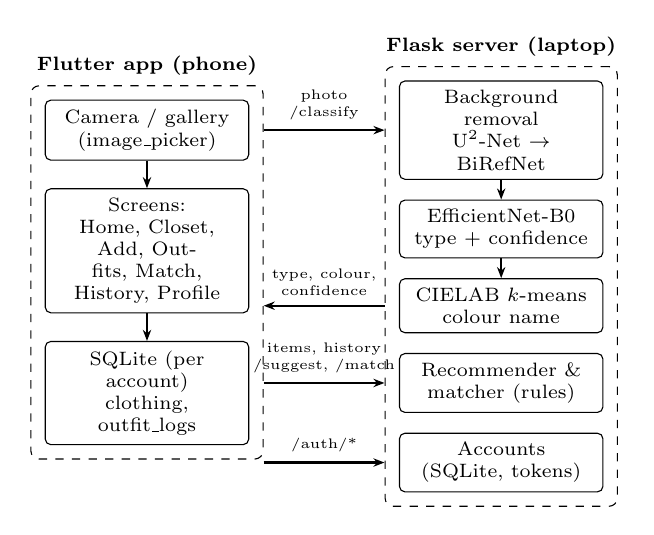
\begin{tikzpicture}[
  font=\scriptsize,
  box/.style={draw, rounded corners=2pt, align=center, minimum height=0.62cm, text width=2.35cm, fill=white},
  grp/.style={draw, dashed, rounded corners=3pt, inner sep=5pt},
  arr/.style={-{Stealth[length=4pt]}, thick}
]
\node[box] (cam) {Camera / gallery\\(image\_picker)};
\node[box, below=0.35cm of cam] (ui) {Screens: Home, Closet,\\Add, Outfits, Match,\\History, Profile};
\node[box, below=0.35cm of ui] (db) {SQLite (per account)\\clothing, outfit\_logs};
\node[grp, fit=(cam)(ui)(db), label={[font=\scriptsize\bfseries]above:Flutter app (phone)}] (app) {};

\node[box, right=1.9cm of cam] (seg) {Background removal\\U\textsuperscript{2}-Net $\rightarrow$ BiRefNet};
\node[box, below=0.25cm of seg] (cls) {EfficientNet-B0\\type + confidence};
\node[box, below=0.25cm of cls] (col) {CIELAB $k$-means\\colour name};
\node[box, below=0.25cm of col] (rec) {Recommender \&\\matcher (rules)};
\node[box, below=0.25cm of rec] (acc) {Accounts\\(SQLite, tokens)};
\node[grp, fit=(seg)(cls)(col)(rec)(acc), label={[font=\scriptsize\bfseries]above:Flask server (laptop)}] (srv) {};

\draw[arr] (cam) -- (ui);
\draw[arr] (ui) -- (db);
\draw[arr] (seg) -- (cls);
\draw[arr] (cls) -- (col);
\draw[arr] (app.east |- seg) -- node[above, font=\tiny, align=center]{photo\\/classify} (srv.west |- seg);
\draw[arr] (srv.west |- col) -- node[above, font=\tiny, align=center]{type, colour,\\confidence} (app.east |- col);
\draw[arr] (app.east |- rec) -- node[above, font=\tiny, align=center]{items, history\\/suggest, /match} (srv.west |- rec);
\draw[arr] (app.east |- acc) -- node[above, font=\tiny]{/auth/*} (srv.west |- acc);
\end{tikzpicture}
\caption{Wardrobe+ architecture. The wardrobe never leaves the phone. Each request carries the items it needs, and the server stores only accounts.}
\label{fig:arch}
\end{figure}

The end-to-end flow is:
\begin{enumerate}
  \item \textbf{Capture.} The user takes or picks a photo. The app copies it into its own storage folder and uploads it as multipart form data.
  \item \textbf{Segment.} The server corrects the EXIF orientation, downsizes the photo to at most 1280\,px and removes the background (Section~\ref{sec:seg}).
  \item \textbf{Classify and colour.} The garment, composited on white, is classified (Section~\ref{sec:cls}), and the colour is detected from the cut-out pixels (Section~\ref{sec:color}).
  \item \textbf{Confirm.} The app shows the predicted type, confidence and colour. The user can correct them before saving, which is also how manually labelled types such as \emph{Outerwear} enter the wardrobe.
  \item \textbf{Wear and recommend.} The user picks an occasion and receives the highest-scoring outfit with reasons (Section~\ref{sec:rec}). Choosing ``Wear this today'' logs the outfit and updates each item's wear count and last-worn date.
\end{enumerate}

%=====================================================================
\section{Implementation}
%=====================================================================
\subsection{Dataset Construction}\label{sec:data}
The training set combines three sources (Table~\ref{tab:data}):
\begin{itemize}
  \item \textbf{Fashion Product Images (Small)}~\cite{kaggleFashion}, 44{,}441 Myntra catalogue images at $60{\times}80$\,px. We take the \texttt{articleType} values \emph{Tshirts}, \emph{Shirts} and \emph{Dresses}, and merge \emph{Jeans} and \emph{Trousers} into a single \emph{Pants} class.
  \item \textbf{Clothing Dataset (full, high resolution)}~\cite{grigorev2020clothing}: crowd-sourced photos of real garments, mostly taken at home, at up to 12\,MP.
  \item \textbf{Team photos}: 156 phone photos of the authors' own clothes.
\end{itemize}

\begin{table}[t]
\caption{Training images per class and source}
\label{tab:data}
\centering
\begin{tabular}{lrrrr}
\toprule
Class & Catalogue~\cite{kaggleFashion} & Clothing DS~\cite{grigorev2020clothing} & Team & Total \\
\midrule
T-shirts & 7{,}066 & 1{,}011 & 85 & 8{,}162 \\
Shirts   & 3{,}215 &   378   & 30 & 3{,}623 \\
Pants    & 1{,}138 &   692   & 31 & 1{,}861 \\
Dresses  &   464   &   357   & 10 &   831   \\
\midrule
Total    & 11{,}883 & 2{,}438 & 156 & 14{,}477 \\
\bottomrule
\end{tabular}
\end{table}

The real-photo sources were added because a model trained only on small catalogue thumbnails generalised poorly to photos taken at home. The classes are imbalanced: there are 9.8 T-shirt images for every dress.

Earlier prototypes also included \emph{Kurtas}, \emph{Jackets} and \emph{Shoes}. Kurtas were dropped because there were too few real photos of them and the model could not recognise them reliably. Jackets and shoes were also dropped. The app still supports \emph{Outerwear} as a type the user sets by hand.

\subsection{Garment Classifier}\label{sec:cls}
We use torchvision's EfficientNet-B0 with ImageNet weights and replace the final linear layer with a 4-way layer. Training uses a stratified split: 15\% of every class (seed 42) is held out for validation. Each training image $i$ with label $y_i$ is drawn by a \texttt{WeightedRandomSampler} with weight
\begin{equation}
  w_i = 1 / n_{y_i},
\end{equation}
where $n_c$ is the number of training images in class $c$. As a result, every class is sampled at roughly the same rate.

To make catalogue images look more like phone photos, we apply heavy augmentation during training: resizing to $256{\times}256$, a random $224{\times}224$ crop, horizontal flips, vertical flips ($p{=}0.1$), colour jitter (brightness and contrast $\pm0.4$, saturation $\pm0.3$, hue $\pm0.1$), rotation of up to $\pm30^\circ$, random greyscale ($p{=}0.05$), ImageNet normalisation and random erasing ($p{=}0.1$). Validation and inference only resize to $224{\times}224$ and normalise.

Training proceeds in two phases (Table~\ref{tab:hyper}). Phase~1 freezes the convolutional features and trains only the classifier head. Phase~2 unfreezes the whole network with a lower learning rate and cosine annealing. The weights from the epoch with the best validation accuracy are kept, and every run is saved as a versioned checkpoint with its metrics.

At inference the server returns the softmax probability of the top class as the confidence, together with the next two classes. The app shows these as alternatives the user can pick.

\begin{table}[t]
\caption{Classifier training configuration}
\label{tab:hyper}
\centering
\begin{tabular}{ll}
\toprule
Parameter & Value \\
\midrule
Backbone & EfficientNet-B0 (ImageNet pretrained) \\
Output classes & 4 (Dresses, Pants, Shirts, T-shirts) \\
Input size & $224\times224$ \\
Batch size & 32 (train), 64 (validation) \\
Loss & Cross-entropy \\
Phase 1 & 5 epochs, head only, Adam, lr = $10^{-3}$ \\
Phase 2 & 10 epochs, all layers, Adam, lr = $10^{-4}$, cosine \\
Class balancing & WeightedRandomSampler, $w_i=1/n_{y_i}$ \\
Validation split & 15\% per class, stratified, seed 42 \\
Hardware & Apple M-series GPU (MPS) \\
\bottomrule
\end{tabular}
\end{table}

\subsection{Two-Stage Background Removal}\label{sec:seg}
U\textsuperscript{2}-Net is fast and accurate on plain backgrounds, but on striped or printed bedsheets it often keeps the sheet or only a logo. Wardrobe+ therefore checks the quality of each mask using two statistics of the alpha channel $\alpha\in[0,255]$:
\begin{equation}
  f = \frac{1}{N}\sum_p [\alpha_p > 160], \qquad
  s = \frac{1}{N}\sum_p [20 < \alpha_p < 235],
\end{equation}
where $[\cdot]$ is 1 when the condition holds and 0 otherwise, $f$ is the foreground share and $s$ is the share of soft, uncertain edge pixels.
A mask that is small or very uncertain is treated as a failure, and the more robust BiRefNet-lite runs instead (Algorithm~\ref{alg:seg}). Both model sessions are created once at server start-up. The cut-out is composited on a white background before classification, which matches the white backgrounds of catalogue images.

\begin{algorithm}[t]
\caption{Garment segmentation with fallback}
\label{alg:seg}
\begin{algorithmic}[1]
\Require photo $I$ (EXIF-corrected, longest side $\le 1280$)
\State $M_1 \gets \textsc{U2Net}(I)$; compute $f_1, s_1$
\If{$f_1 \ge 0.25$ \textbf{and} $s_1 \le 0.10$}
  \State \Return $M_1$
\EndIf
\State $M_2 \gets \textsc{BiRefNetLite}(I)$; compute $f_2$
\If{$f_2 > f_1$} \Return $M_2$ \Else\ \Return $M_1$ \EndIf
\end{algorithmic}
\end{algorithm}

\subsection{Colour Detection}\label{sec:color}
Only garment pixels with $\alpha>160$ are used, and at most 6{,}000 of them are sampled at random. The pixels are converted to CIELAB, where lightness $L^*$ is separate from the chromatic axes $a^*,b^*$. For each colour we compute the chroma and hue angle:
\begin{equation}
  C = \sqrt{a^{*2}+b^{*2}}, \qquad h = \operatorname{atan2}(b^*, a^*) \bmod 360^\circ.
\end{equation}
OpenCV $k$-means with $k{=}3$, $k$-means++ seeding~\cite{arthur2007kmeanspp} and 4 restarts clusters the pixels, and the clusters are sorted by size. The largest cluster centre is named by a rule-based decision on $(L^*, C, h)$ into one of 18 colour names. Two ranges of the rules handle common phone-photo effects:
\begin{itemize}
  \item Low-chroma, warm-hued centres ($C<22$, $50^\circ\le h\le110^\circ$) are white, beige or brown depending on $L^*$, because white fabric appears yellowish under indoor light.
  \item Near-neutral centres with a faint blue hue ($2.5\le C<8$, $200^\circ\le h\le300^\circ$) are named light blue or navy, because that is how denim looks in photos.
\end{itemize}
An item is labelled \emph{multicolour} if a second or third cluster covers at least 22\% of the pixels and is clearly a different colour from the largest one. Two centres count as different if:
\begin{itemize}
  \item both are chromatic ($C>18$) and their hues differ by more than $60^\circ$,
  \item only one is chromatic and their CIELAB distance exceeds 45, or
  \item both are neutral and their lightness differs by more than 55 (e.g.\ a black-and-white print).
\end{itemize}
These conditions keep shadows on a plain garment from being labelled as a second colour.

\subsection{Outfit Recommendation}\label{sec:rec}
\textbf{Candidates.} For an occasion $o\in\{\text{Casual, Office, Party, Travel}\}$, the candidate outfits are every top--pants pair and every dress, using only items whose type is allowed for $o$. For Office and Travel, each candidate may also get an outerwear layer if the layer's colour score with the main piece is at least 0.8. Items worn in the last two days are excluded unless nothing else is left.

\textbf{Score.} Each candidate outfit $\mathcal{O}$ is scored as
\begin{equation}
  S(\mathcal{O}) = \operatorname{clip}_{[0,1]}\big(0.35\,H + 0.30\,F + 0.35\,O - P\big).
  \label{eq:score}
\end{equation}
\emph{Colour harmony} $H$ is the pairwise colour score of the main piece with the pants (and with the layer, averaged), taken from Table~\ref{tab:harmony}. A dress alone gets $H=0.85$. Blue and light-blue pants are treated as neutral denim.

\emph{Freshness} is the mean over items of
\begin{equation}
  F_j = \min(d_j/14,\,1),
\end{equation}
where $d_j$ is the number of days since item $j$ was last worn. Items that have never been worn get $F_j=1$.

\emph{Occasion fit} is $O = 0.7\,T + 0.3\,M$. Here $T$ is the type suitability of the main piece from Table~\ref{tab:occasion}. When a layer is present, $T$ is a blend of 0.8 of the main piece's suitability and 0.2 of the layer's. $M$ is the colour mood: it weights the main piece's colour by 0.55 and the mean of the other pieces' colours by 0.45. For example, Office prefers muted colours and Party prefers bold ones.

The \emph{repeat penalty} $P$ is 0.25 if the identical outfit was logged within the past 7 days, 0.10 within 30 days, and 0 otherwise.

\begin{table}[t]
\caption{Pairwise colour-harmony rules}
\label{tab:harmony}
\centering
\begin{tabular}{lc}
\toprule
Pair of colours & Score \\
\midrule
Neutral + chromatic colour & 1.00 \\
Two different neutrals & 0.90 \\
Print (multicolour) + neutral & 0.90 \\
Listed complementary pair (e.g.\ brown/olive, pink/light blue) & 0.80 \\
Same neutral (tonal) & 0.70 \\
Same chromatic colour & 0.55 \\
Unknown colour & 0.50 \\
Two unrelated chromatic colours & 0.35 \\
Print + chromatic colour & 0.30 \\
Two prints & 0.15 \\
\bottomrule
\end{tabular}
\end{table}

\begin{table}[t]
\caption{Type suitability $T$ per occasion (0 removes the item)}
\label{tab:occasion}
\centering
\begin{tabular}{lcccc}
\toprule
Type & Casual & Office & Party & Travel \\
\midrule
T-shirt   & 1.00 & 0.00 & 0.35 & 1.00 \\
Shirt     & 0.65 & 1.00 & 0.75 & 0.55 \\
Dress     & 0.75 & 0.55 & 1.00 & 0.45 \\
Pants     & 1.00 & 1.00 & 1.00 & 1.00 \\
Outerwear & 0.60 & 1.00 & 0.00 & 0.80 \\
\bottomrule
\end{tabular}
\end{table}

\textbf{Ranking and diversity.} Candidates are sorted by $S$. A layered outfit gets a +0.03 tie-break bonus that is not shown to the user. When the user asks for another look, outfits already shown are skipped, and the rest are re-ranked with a penalty of 0.10 for each time one of their pieces has already appeared. This way the next suggestion changes the main piece, not only the pants. The percentage shown in the app is $100\cdot S$.

\textbf{Explanations.} Each component that contributes to the score adds a sentence to the explanation, for example ``Navy grounds the red'', ``The white shirt hasn't been worn in 21 days'', ``Shirt suits office'' or ``You wore this exact outfit 3 days ago''.

\subsection{Find a Match}
Given one top or one pair of pants $a$, every item $b$ of the opposite kind is ranked by
\begin{equation}
  S_{\text{pair}} = 0.45\,\tilde H + 0.25\,Y + 0.15\,F_b + 0.15\,O - P.
\end{equation}
If no occasion is selected, the weights become 0.55, 0.30, 0.15 and 0. Colour combines harmony with light/dark contrast: $\tilde H = 0.75\,H + 0.25\,K$, where $K=\min(|L_a-L_b|/40,1)$ and $L$ is a nominal $L^*$ value for each colour name.

Style compares how dressy the two pieces are, with formality $\phi$ = 0.25 for a T-shirt, 0.8 for a shirt, 0.3 for denim pants, 0.7 for dark or neutral pants and 0.5 otherwise. With $g=\phi_{\text{top}}-\phi_{\text{pants}}$,
\begin{equation}
  Y = \begin{cases} 1 - 0.5\,g, & g>0\\ 1 - 0.8\,|g|, & g\le 0 \end{cases}
\end{equation}
so a dressier top over jeans (smart casual) costs less than a T-shirt with formal trousers. Items worn in the last two days are listed last and marked as recently worn.

\subsection{REST API}
The Flask server exposes the endpoints in Table~\ref{tab:api}. Account data lives in a server-side SQLite database. Passwords are stored as salted scrypt hashes, and logging in returns a random 256-bit token that must accompany every photo and outfit request as a bearer token. The \texttt{/suggest} and \texttt{/match} requests carry the relevant items and wear history from the phone, so the server keeps no per-user wardrobe state.

\begin{table}[t]
\caption{REST endpoints}
\label{tab:api}
\centering
\begin{tabular}{>{\raggedright\arraybackslash}p{2.6cm}>{\raggedright\arraybackslash}p{5.1cm}}
\toprule
Endpoint & Purpose \\
\midrule
GET \texttt{/health} & Status, model classes, supported types, colours, occasions \\
POST \texttt{/auth/register}, \texttt{/auth/login}, \texttt{/auth/logout}, GET \texttt{/auth/me} & Account management; login returns a bearer token \\
POST \texttt{/classify} & Image $\rightarrow$ type, confidence, two alternatives, colour, segmenter used \\
POST \texttt{/suggest} & Items, occasion, history $\rightarrow$ best outfit, match score, score breakdown, reasons \\
POST \texttt{/match} & Anchor item, items, optional occasion $\rightarrow$ ranked partners with reasons \\
\bottomrule
\end{tabular}
\end{table}

\subsection{Mobile Application}
The Flutter (Dart) client targets Android and iOS from one codebase and has five tabs: Home, Closet, Add, Outfits and Profile. It also has screens for clothing details, find a match, outfit history and server settings.

\begin{itemize}
  \item \textbf{Home} shows today's outfit, recently added pieces and pieces not worn for two weeks or more.
  \item \textbf{Closet} filters items by type. Each item's detail page shows how many times it has been worn, when it was last worn and when it was added, and the type and colour can be edited there.
  \item \textbf{Storage.} Each account has its own SQLite file with two tables: \texttt{clothing} (type, colour, confidence, image file name, date added, last worn, wear count) and \texttt{outfit\_logs} (date, item ids, occasion). Photos are copied into the app's documents folder, and only file names are stored, so the paths stay valid across app updates.
  \item \textbf{Server address.} The address is configured in the app, and the server prints its local network name at start-up.
\end{itemize}

\subsection{Technology Stack and Testing}
Table~\ref{tab:stack} lists the stack. The backend logic is covered by 47 unit tests: colour naming, the recommender, the matcher and accounts. The app has 25 unit tests for the database, helpers and profiles, plus an end-to-end integration test that adds real photos through the running server and generates outfits.

\begin{table}[t]
\caption{Technology stack}
\label{tab:stack}
\centering
\begin{tabular}{ll}
\toprule
Component & Technology \\
\midrule
Deep learning & PyTorch 2.10, torchvision 0.25 \\
Classifier & EfficientNet-B0 (fine-tuned) \\
Segmentation & rembg: U\textsuperscript{2}-Net, BiRefNet-general-lite (ONNX) \\
Colour & OpenCV $k$-means in CIELAB, NumPy \\
Web server & Flask 3.1, flask-cors, Werkzeug (scrypt) \\
Mobile app & Flutter (Dart): http, image\_picker, sqflite \\
Storage & SQLite (device: wardrobe; server: accounts) \\
Training hardware & Apple M-series GPU via MPS \\
\bottomrule
\end{tabular}
\end{table}

%=====================================================================
\section{Results and Evaluation}
%=====================================================================
\subsection{Validation Accuracy}
The classifier was trained with the configuration in Table~\ref{tab:hyper} on 12{,}307 images, and 2{,}170 images were held out for validation. The best validation accuracy, 98.5\%, was reached in phase~2, epoch~6 (epoch 11 overall). Fig.~\ref{fig:curve} shows the training curves, and Table~\ref{tab:val} gives the results per class and per source.

Accuracy on the catalogue images is the highest. This is expected, because catalogue images are uniform and near-duplicate products can fall on both sides of a random split. The real-photo subsets are the more meaningful indicator of how the model behaves inside the app.

\begin{figure}[t]
\centering
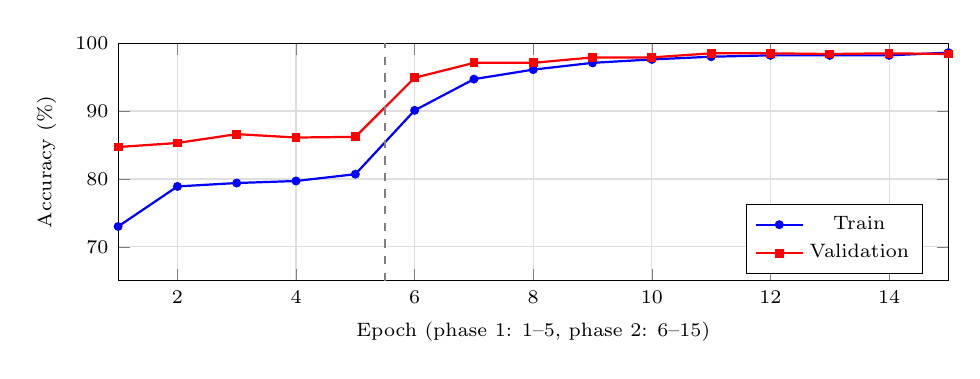
\begin{tikzpicture}
\begin{axis}[
  width=\columnwidth, height=4.6cm,
  xlabel={Epoch (phase 1: 1--5, phase 2: 6--15)}, ylabel={Accuracy (\%)},
  xmin=1, xmax=15, ymin=65, ymax=100,
  legend pos=south east, legend style={font=\scriptsize},
  tick label style={font=\scriptsize}, label style={font=\scriptsize},
  grid=major, grid style={gray!25}
]
\addplot[thick, blue, mark=*, mark size=1.2pt] coordinates {(1,73.0)(2,78.9)(3,79.4)(4,79.7)(5,80.7)(6,90.1)(7,94.7)(8,96.1)(9,97.1)(10,97.6)(11,98.0)(12,98.2)(13,98.2)(14,98.2)(15,98.6)};
\addlegendentry{Train}
\addplot[thick, red, mark=square*, mark size=1.2pt] coordinates {(1,84.7)(2,85.3)(3,86.6)(4,86.1)(5,86.2)(6,94.9)(7,97.1)(8,97.1)(9,97.9)(10,97.9)(11,98.5)(12,98.5)(13,98.4)(14,98.5)(15,98.4)};
\addlegendentry{Validation}
\draw[dashed, gray] (axis cs:5.5,65) -- (axis cs:5.5,100);
\end{axis}
\end{tikzpicture}
\caption{Training and validation accuracy. Training accuracy is measured on augmented, class-balanced batches, so it can be lower than validation accuracy.}
\label{fig:curve}
\end{figure}

\begin{table}[t]
\caption{Validation accuracy (\%) by class and by source}
\label{tab:val}
\centering
\begin{tabular}{lrrrr}
\toprule
Class & Images & All & Catalogue & Real photos\textsuperscript{a} \\
\midrule
Dresses & 124 & 98.4 & 100.0 & 96.6 \\
Pants & 279 & 100.0 & 100.0 & 100.0 \\
Shirts & 543 & 99.8 & 99.8 & 100.0 \\
T-shirts & 1{,}224 & 97.6 & 98.2 & 93.9 \\
\midrule
Overall & 2{,}170 & 98.5 & 98.9 & 96.8 \\
\bottomrule
\multicolumn{5}{l}{\footnotesize \textsuperscript{a}Clothing Dataset~\cite{grigorev2020clothing} and team photos combined.}
\end{tabular}
\end{table}

\begin{table}[t]
\caption{Validation confusion matrix (rows: true, columns: predicted)}
\label{tab:confusion}
\centering
\begin{tabular}{lrrrr}
\toprule
 & Dresses & Pants & Shirts & T-shirts \\
\midrule
Dresses & 122 & 0 & 1 & 1 \\
Pants & 0 & 279 & 0 & 0 \\
Shirts & 0 & 0 & 542 & 1 \\
T-shirts & 13 & 4 & 12 & 1195 \\
\bottomrule
\end{tabular}
\end{table}

Table~\ref{tab:confusion} shows that almost all remaining errors (29 of 32) are true T-shirts. They are predicted as dresses, shirts or, less often, pants. T-shirts are also the weakest class on real photos, with 93.5\% accuracy on the Clothing Dataset images. Long or loose T-shirts photographed flat can resemble short dresses, and the boundary between a T-shirt and a casual shirt is not always clear even to annotators.

\subsection{Held-Out Real Wardrobe Photos}
The validation split still contains images drawn from the same sources and photo sessions as the training data. We therefore also evaluate the complete app pipeline (segmentation, classification and colour) on 12 phone photos of the team's clothes that are not in the training data, with labels written down in advance (Table~\ref{tab:holdout}).

The deployed model, trained on all 14{,}477 images, classifies all 11 garments of supported types correctly, with a median confidence of 100\%. The twelfth photo is a kurta, which the model does not support, and it is excluded from the type score. The colour is correct for all 12 photos. The model from the validation run in Section~V-A, which never saw 15\% of the data, scores 10/11 for type and 12/12 for colour on the same set. Its one error is a white shirt predicted as a dress with 95\% confidence. This shows that two models trained with the same recipe can differ on individual photos, and that a high confidence does not guarantee a correct answer.

Both models also label the kurta as a \emph{Dress} with more than 99\% confidence. A closed-set classifier has no way to say ``none of these'', so the app always shows the prediction for the user to confirm or correct. Out-of-distribution detection is left for future work.

Two caveats apply. With only 11 or 12 photos, a single error changes the accuracy by about 9 points. The colour thresholds were also tuned while inspecting these same photos, so the colour score is optimistic.

\begin{table}[t]
\caption{Full pipeline on 12 held-out real photos (deployed model)}
\label{tab:holdout}
\centering
\begin{tabular}{>{\raggedright\arraybackslash}p{2.4cm}>{\raggedright\arraybackslash}p{2.2cm}>{\raggedright\arraybackslash}p{2.6cm}}
\toprule
Task & Result & Notes \\
\midrule
Type (supported classes) & 11/11 & 1 kurta excluded (unsupported class) \\
Colour & 12/12 & rules tuned on this set \\
Segmenter used & U\textsuperscript{2}-Net 9, BiRefNet 3 & fallback on busy backgrounds \\
\bottomrule
\end{tabular}
\end{table}

\subsection{Correction of an Earlier Evaluation}
An earlier version of this work reported 98--100\% test accuracy. That figure was invalid. The test script copied randomly chosen images out of the training folder, so the model was evaluated on images it had trained on. The current training script records its held-out validation files inside the checkpoint, and evaluation on real photos uses a separate set that is checked not to overlap with the training data. All numbers in this section come from these corrected procedures.

\subsection{Latency}
On an Apple M4 laptop CPU, one classification request (segmentation, classification and colour) takes about 0.4\,s when U\textsuperscript{2}-Net is accepted and about 6\,s when the BiRefNet fallback runs. The first request after start-up also downloads the segmentation models (about 400\,MB, once). Outfit scoring is plain Python and takes milliseconds for wardrobes of a few hundred items.

%=====================================================================
\section{Limitations and Future Work}
%=====================================================================
\begin{itemize}
  \item \textbf{Classes.} The model recognises only four garment types. Outerwear is labelled by hand, and kurtas are not supported. Adding them requires a few hundred real photos per class. Unsupported garments are confidently forced into one of the four classes, which an out-of-distribution check could flag.
  \item \textbf{Evaluation scale.} The held-out set of real photos is small. We plan to collect a larger, independently labelled set and to report colour accuracy on photos that were not used to tune the rules.
  \item \textbf{Recommendation.} The rules encode general styling heuristics rather than personal taste. Learning from the outfits a user accepts or skips, weather-aware suggestions and pattern detection are planned.
  \item \textbf{Accessibility.} Spoken garment descriptions and voice navigation for visually impaired users are planned and are not part of the current app.
  \item \textbf{Deployment.} Wardrobes are stored only on the phone and do not sync across devices. The server is reached over plain HTTP on the local network, which is suitable for development only.
\end{itemize}

%=====================================================================
\section{Conclusion}
%=====================================================================
Wardrobe+ shows that a useful wardrobe assistant can be built from a phone camera, a laptop-class server and off-the-shelf models. Key to making it work on real photos were a segmenter that falls back to a more robust model on cluttered backgrounds, training data that includes real photos and not only catalogue images, colour rules adapted to indoor lighting, and an evaluation that is not contaminated by training data. The rule-based recommender keeps every suggestion explainable and nudges users toward clothes they already own but rarely wear. This is a small, concrete step toward wearing clothes more often and buying fewer.

\section*{Acknowledgment}
The authors thank Prof. Neha Ram for her guidance, and the creators of the Fashion Product Images and Clothing datasets for making them publicly available.

\begin{thebibliography}{99}

\bibitem{emf2017}
Ellen MacArthur Foundation, ``A new textiles economy: Redesigning fashion's future,'' 2017. [Online]. Available: https://www.ellenmacarthurfoundation.org/a-new-textiles-economy

\bibitem{liu2016deepfashion}
Z.~Liu, P.~Luo, S.~Qiu, X.~Wang, and X.~Tang, ``DeepFashion: Powering robust clothes recognition and retrieval with rich annotations,'' in \emph{Proc. IEEE CVPR}, 2016, pp.~1096--1104.

\bibitem{kiapour2015street2shop}
M.~Hadi~Kiapour, X.~Han, S.~Lazebnik, A.~C.~Berg, and T.~L.~Berg, ``Where to buy it: Matching street clothing photos in online shops,'' in \emph{Proc. IEEE ICCV}, 2015, pp.~3343--3351.

\bibitem{ji2020pipeline}
Y.-H.~Ji \emph{et al.}, ``An effective pipeline for a real-world clothes retrieval system,'' arXiv:2005.12739, 2020.

\bibitem{goh2011smart}
K.~N.~Goh, Y.~Y.~Chen, and E.~S.~Lin, ``Developing a smart wardrobe system,'' in \emph{Proc. IEEE Consumer Communications and Networking Conf. (CCNC)}, 2011, pp.~303--307.

\bibitem{banoth2022nextgen}
R.~Banoth, A.~G.~Godishala, H.~Yassin, and V.~Raj, ``Next generation smart wardrobe management system using IoT,'' in \emph{Proc. IEEE Int. Conf. for Convergence in Technology (I2CT)}, 2022.

\bibitem{he2016resnet}
K.~He, X.~Zhang, S.~Ren, and J.~Sun, ``Deep residual learning for image recognition,'' in \emph{Proc. IEEE CVPR}, 2016, pp.~770--778.

\bibitem{tan2019efficientnet}
M.~Tan and Q.~V.~Le, ``EfficientNet: Rethinking model scaling for convolutional neural networks,'' in \emph{Proc. ICML}, 2019, pp.~6105--6114.

\bibitem{deng2009imagenet}
J.~Deng, W.~Dong, R.~Socher, L.-J.~Li, K.~Li, and L.~Fei-Fei, ``ImageNet: A large-scale hierarchical image database,'' in \emph{Proc. IEEE CVPR}, 2009, pp.~248--255.

\bibitem{qin2020u2net}
X.~Qin, Z.~Zhang, C.~Huang, M.~Dehghan, O.~R.~Zaiane, and M.~Jagersand, ``U\textsuperscript{2}-Net: Going deeper with nested U-structure for salient object detection,'' \emph{Pattern Recognition}, vol.~106, p.~107404, 2020.

\bibitem{zheng2024birefnet}
P.~Zheng, D.~Gao, D.-P.~Fan, L.~Liu, J.~Laaksonen, W.~Ouyang, and N.~Sebe, ``Bilateral reference for high-resolution dichotomous image segmentation,'' \emph{CAAI Artificial Intelligence Research}, vol.~3, 2024.

\bibitem{rembg}
D.~Gatis, ``rembg: Rembg is a tool to remove images background,'' GitHub repository. [Online]. Available: https://github.com/danielgatis/rembg

\bibitem{han2017bilstm}
X.~Han, Z.~Wu, Y.-G.~Jiang, and L.~S.~Davis, ``Learning fashion compatibility with bidirectional LSTMs,'' in \emph{Proc. ACM Multimedia}, 2017, pp.~1078--1086.

\bibitem{cui2019nodewise}
Z.~Cui, Z.~Li, S.~Wu, X.~Zhang, and L.~Wang, ``Dressing as a whole: Outfit compatibility learning based on node-wise graph neural networks,'' in \emph{Proc. The Web Conference (WWW)}, 2019, pp.~307--317.

\bibitem{arthur2007kmeanspp}
D.~Arthur and S.~Vassilvitskii, ``k-means++: The advantages of careful seeding,'' in \emph{Proc. ACM-SIAM SODA}, 2007, pp.~1027--1035.

\bibitem{kaggleFashion}
P.~Aggarwal, ``Fashion Product Images (Small),'' Kaggle, 2019. [Online]. Available: https://www.kaggle.com/datasets/paramaggarwal/fashion-product-images-small

\bibitem{grigorev2020clothing}
A.~Grigorev, ``Clothing dataset (full, high resolution),'' Kaggle, 2020. [Online]. Available: https://www.kaggle.com/datasets/agrigorev/clothing-dataset-full

\end{thebibliography}

\end{document}
